\section{Introduction}
The movie industry continues to grow year on year, with increasing competition between movie producers and film companies to boost revenue and increase ratings. The performance of a movie at the box office is influenced by a host of factors, some of which include the cast, budget, time of release and director involved. This makes predicting the box office of movies very challenging. Quite a number of studies, however, have been done by many researchers attempting to identify the influential factors and predict the box office of movies \cite{sharda2006predicting}. Most of the studies failed to build models with high predicting accuracy that can serve as guidelines for decision making process. Most of the literature on this problem can be classified into two categories i) predicting the gross prior to movie release; ii) predicting the gross after the movie release. Models built in the second category generally have higher precision as more predictive variables including first week box office and word-of-mouth effects are provided. Besides, all the studies turned this problem into classification problem as the value of movie gross is very sparse.  And many traditional statistical methods and artificial neural network (ANN) were applied. Among those methods, ANN performed the best with highest accuracy under the same experimental conditions \cite{sharda2006predicting}.
 
The aim of our study is to apply different kinds of predictive data mining techniques including classification and regression and try to find the best model. What differentiates our study from the others is that we first built a classification model and then used the predicting results of the classification model as new features for regression models. Results show there is a 10\% increase in regression model accuracy. Besides, for each category from the classification model, we once again performed all the techniques and find the best model for each category.


\section{Materials and methods}

\subsection{IMDB dataset}
The dataset used was the IMDB 5000 Movie Dataset hosted on Kaggle \footnote{https://www.kaggle.com/deepmatrix/imdb-5000-movie-dataset}. It has the data for 5044 movies, ordered by the highest grossing values and it provides 28 features. Features range from binary values (colour or black and white), textual (director and actor names, genre, country of origin) as well as numerical values (gross, number of likes on social media, release year).  However, the dataset had several limitations, one of which is missing values. For this reason, we performed the scraping process again to improve the dataset and collect more data that was originally available.

\subsubsection{Re-scraping}
First, up-to-date budget values were sourced from the-numbers.com, which provides a database of production and marketing budgets for movies, as well as domestic and worldwide gross values. The original dataset only included the domestic gross estimates from IMDB.com, which are severely lacking and for majority of popular films omit large portions of revenue that was earned in other countries.  As the worldwide gross is the target value that was being predicted, and ultimately that measured the success of the models presented, it was important to get this feature right.

Secondly, based on the list of movies obtained in the first step, the script obtained the IMDB links for the movies, using fuzzy matching (as some movies have several names that identify them, eg. Fast \& Furious 6 and Furious 6) to resolve naming ambiguities, and scraped IMDB for the available data about genre, actors, year and other important features. Additionally, the script queried the Facebook for popularity measures, count of likes for actors, movies and directors.

\subsubsection{Dataset joining}
Finally, data from all steps, the-numbers.com, IMDB and Facebook, was joined in a single dataset ordered by highest grossing movies. Other than the resolving most of the missing values and updating the information, the main contribution of this step was the correction of worldwide gross values. Additionally, all values were converted to a common currency (USD), as the original dataset reported gross values in local currencies. This was particularly important for currencies that have low exchange rate to USD, like South Korean Won. Gross values reported in those currencies had artificially high numbers due to the exchange rate of their currency compared to USD.


\subsection{Feature engineering}
In order to properly understand the data and see the performance of models in later stages, feature engineering is an important step that must be performed initially to ensure that irregularities are not negatively affecting the performance.

Since our goal is to predict box-office revenue before the movie premiere, the first step was to remove the features that are not available before the release of the movie. Those include \textit{imdb\_score, movie\_facebook\_likes, num\_critic\_for\_reviews, \\num\_user\_for\_reviews, num\_voted\_users}, as they, although present in the dataset, should not be included in models that deal with prediction.

After obtaining the updated and improved dataset, additional work was performed manually to clean and enhance the data. Duplicates were removed, and additional columns were added, like ‘blockbuster’, which designated is the movie released during Christmas or Summer season (June/July/August/December), as well as manual fixing of duration, countries, and similar values that show outliers. Some movies, for example, have lengths of close to 10 hours, and all these tasks were performed by OpenRefine.

\subsubsection{Data transformations}
Additionally, in cases where there is a lot of differences in variation in a dataset, data can be classified as heteroscedastic. Logarithmic transformation is usually applied in those situations \cite{kvalheim1994preprocessing}. Given that the ranges for the worldwide gross are several orders of magnitude, from hundreds of thousands of dollars, all the way to billions, logarithmic transform in this case solves the issue.

In the pipeline process, several other transformations were applied as well, like standardisation, normalisation and polynomial transformation. Those were proved to be useful depending on the model. However, polynomial did not contribute any improvement in scores but did increase the complexity significantly, so it was not explored after initial experimentation.

Finally, categorisation of the data was performed to handle non-numerical data. Results were compared to find the combination of transformers that provides the best scores. The resulting combination was the following: count vectoriser was used for name values (actors and directors) and term-frequency was applied to categorical values (like colour, countries, genres). The differences between different approaches are minor, less than 1% (second best combination was 0.73% less accurate, it used count vectoriser for names and term-frequency/inverse-document-frequency for categorical values), but still affect the end model so it was important to find the best performing transformations.


\subsection{EXPLORATORY DATA ANALYSIS (EDA)}
We applied Exploratory Data Analysis aiming to understand the nature of the data, bivariate relationships and discover patterns that can guide the selection and application of prediction machine learning techniques \cite{behrens1997principles}. FIGURE(a) shows that gross variable is not normally distributed. Therefore, it is useful to use the logarithmic transformation to deal with a more normally distributed version of this variable. See FIGURE(b). A similar exploration analysis was applied on the other variables using the common visualization tools, including pairwise plots and correlations matrix. Correlation analysis revealed that gross and budget are positively correlated (correlation coefficient of 0.74), and that there is not a significant correlation between the movie gross and the other explanatory variables. FIGURE(a) and FIGURE(b), which present a scatter plot of the two most relevant variables in their original and log transformed form, illustrate that these variables are highly heteroscedastic. 

\subsubsection{DIMENSIONALITY REDUCTION}
A plot of the cumulative explained variance plot created by means of PCA over the processed dataset is shown in FIGURE, where it can be seen that there is not a small subset of variables that can explain the majority of variance in the data. In other words, we need 125 variables (out of 184) to explain 80% of the variation. This means that there is not much space for dimensionality reduction in this dataset.

FIGURE: Explained variance plot.

Dimensionality reduction is also useful to create a visual representation of multidimensional data in a reduced space. For instance, FIGURE shows a PCA-reduced 3D representation of the dataset studied in this report. From FIGURE it can be seen that most of the observations are scarcely scattered in a certain area of the plot, but also there is a considerable amount of points scattered outside that area. FIGURE also shows that there is not clear evidence of clusters. 

FIGURE: PCA-reduced 3D visualization of the dataset

Regarding feature selection, we tried several methods such as variance threshold, recursive feature elimination, and feature selection based on models. As expected, all these methods agree that the most important variables are the numeric variables. However, they differ in which of the binary variables are the most relevant.



\subsection{APPROACH}
\subsubsection{Pipeline}
The pipeline was built on top of sklearn’s Pipe and Gridsearch functions. It’s architecture was more advanced in comparison with original Pipe, as it supported a search of different models and not only the parameters.

We aimed to find the most accurate model among different machine learning techniques including regressions, logistic regression, random forest and neural net. For each model, we also needed to set a range values for each parameter in order to fine-tune the model.
 
Also, before our data was fed into the models, we performed numerous pretreatment methods towards the data, i.e. transformation, scaling and dimension reduction.
 
The workflow applied in this project is shown in FIGURE. In order to integrate and automate this workflow (excluding data collecting), we used a function called pipeline in sklearn \cite{sklearnpipeline}, which allows us to set parameters for algorithms in each step while chaining them together without keeping track of the data.


However, parameters in each model have different potential values and there are many different combinations of the parameters in between the workflows. All the values and combinations should be tested in order to find the most optimal one.
 
These processes of setting values and trying combinations can be tedious. GridSearchCV in sklearn allows us to construct a grid of the combinations and search for the best one. Besides, it also automatically performs cross-validation on each model for each combination. In the end, it returns the best model and best parameters. The price of these benefits, however, is in the form of computation time. A pipeline trying different pre-processing, transformation, reducers, and parameter grids,  can take several hours to complete. 



\subsection{REGRESSION}
A number of regression techniques were applied to the problem via the pipeline, with varying results. Based on insights from our experimentation, focus was placed on one regression technique: Gradient Boosting Regression.  This section describes in detail the application of this method ensemble method in predicting gross values of movies. 



\subsubsection{Gradient Boosting Regression}
Gradient Boosting was applied on the data, with least squares as the error function. The best result was produced with a Gradient Boosting Regressor with 1000 base learners and a corresponding low learning rate of 0.1. Base learners in this case are decision trees which are used as weak learners in the gradient boosting process \cite{natekin2013gradient}. These are constructed in a greedy fashion, choosing the best split to minimize the loss. 

Given the high number of regression trees combined to form the Gradient Boosting model, a visual inspection of individual trees is hard to interpret. We look into feature importance to highlight features that would ordinarily be used frequently in split points in our model. It is found that the most important features for this model are the production budget,  movie duration, and the total number of Facebook likes for the cast. The production budget however immensely outweighs the other features in terms of importance. 

To extend this further, we take a look at partial dependence plots to show the dependence between the target response and the most important set of features (i.e. the expected response as a function of the features). Figure shows dependency plots for total number of Facebook likes, movie duration and production budget. The lower left plot shows the effect the production budget has on the movie gross, and it can be seen that there is a linear relationship between them. The lower right plot shows the interactions among the production budget and movie duration, which are the two most important features as per the model. For a movie of a certain duration d (both high and low durations), its gross is strongly dependent on production budget.  The remaining two plots, point to the fact that there is not a strong linear relationship between the target variable and the Facebook likes of cast and movie duration.



FIGURE:     


We also plot a learning curve to provide some insight into training and validation scores for varying number of training samples. From Figure  it can be seen that the training and validation performance do not converge for as the number of training samples increases. This indicates that addition of  more data will likely help increase the validation performance as well as model generalization to new data.


Figure

\subsubsection{CLASSIFICATION}

\subsubsection{Classification Analysis}
Over a dozen different classifiers have been used within the pipeline. As result of experimentation, the pipeline was narrowed down to one classifier. This section discusses the optimization of parameters for selecting the right model to grow the decisions trees and constructing the ensembles to generalize a well fitted model, taking into account bias/variance trade-off \cite{biasvariance}. Overall, 9 different classification cases were attempted, ranging from classifying into 2 classes up to 10 classes of gross values. 









FIGURE: Plot pairwise relationships between selected features created with the seaborn python library.


\subsubsection{Dimensionality reduction}
The cumulative explained variance plot created by means of PCA over the processed dataset is shown in FIGURE, where it can be seen that there is not a small representative subset of variables that can explain the majority of variance in the data. In other words, 125 variables (out of 184) explain 80% of the variation. This means that there is not much space for dimensionality reduction in this dataset.

FIGURE: Explained variance plot.



Dimensionality reduction is also useful to create a visual representation of multidimensional data in a reduced space. For instance, FIGURE shows a PCA-reduced 3D representation of the dataset studied in this report. From FIGURE it can be drawn that most of the observations are scarcely scattered in a certain area of the plot, but also there is a considerable amount of points scattered outside that area. FIGURE also shows that there is not clear evidence of clusters. 

FIGURE: PCA-reduced 3D visualization of the dataset

\subsubsection{Approach}
The \textbf{pipeline} was built on top of sklearns Pipe and Gridsearch functions. It’s architecture was more advanced in comparison with original Pipe, as it supported a search of different models and not only the parameters.

We aim to find the most accurate model among different algorithms including regressions, logistic regression, random forest and neural net. For each model, we also need to set different values for each parameter in order to fine-tune the model.
 
Besides, before our data fed into the models, we performed numerous pretreatment methods towards the data, i.e. transformation, scaling and dimension reduction.
 
The workflows applied in this project is shown in figure1. In order to integrate and automate this workflows (excluding data collecting), we used a function called Pipeline in Scikit-learn, which allows us to set parameters for algorithms in each step while chaining them together without keeping track of the data.

However, each parameter in each model have different potential values and there are many different combinations of the parameters in between the workflows. All the values and combinations should be tested in order to find the most optimal one.
 
These processes of setting values and trying combinations can be tedious. GridSearchCV in Scikit-learn allows us to construct a grid of the combinations and search for the best one. Besides, it also automatically performs cross-validation on each model for each combination. In the end, it returns us with the best model and best parameters.

\textbf{Linear and Logistic Regressions:}
An ordinary linear regression model is a common starting point for analysis since its results can serve as a baseline for any further data analysis. The dependent variable, which is the movie gross, can be predicted using the multivariate linear regression. The highly correlatable predictors, such as number of Facebook likes, IMBD score and number of reviews will be used to build a robust regression model. Later on, we can aggregate those factors by giving each of them a weight and then use below mentioned neural network technique to fine-tune the weights. Some other regression models, like k-nearest neighbour algorithm and multinomial logistic regression will be explored as well.

\textbf{Decision trees:}
Classification and Regression Trees (CART) trees could be another technique that apply in this case. Seeing as decision trees are able to handle both categorical and numerical data, there is the flexibility is drawing comparisons between both classification and regression.  Random Forests will also be considered in this case in order to add diversity to the decision tree models. 

\textbf{Neural Networks:}
Neural networks approach is useful in these types of problems where there is a lot of features, and based on data obtained from previous techniques, we will experiment with neural networks algorithms to see how they behave. Those include simpler neural networks, like feed-forward NN, to more complex ones, like recursive NN, which might show some additional insight.

By applying those techniques, we aim to build a successful model that accepts certain movie related factors and predicts the box-office and its rating. Additionally, we will compare the performance of the aforementioned machine learning techniques when predicting the box-office. We are also interested in assessing the performance of Ensemble Learning, which combines multiple models to cancel the systematic bias of individual forecast models. Gradient Boosting, an example of this approach, has proved to be effective in some of the last Kaggle competitions..
\section{Regression}
\subsection{Gradient Boosting Regression}
Gradient Boosting was applied on the data, with least squares as the error function. The best result was produced with a Gradient Boosting Regressor with 1000 base learners and a corresponding low learning rate of 0.1. Base learners in this case are decision trees which are used as weak learners in the gradient boosting process \cite{natekin2013gradient}. These are constructed in a greedy fashion, choosing the best split to minimize the loss. 

Given the high number of regression trees combined to form the Gradient Boosting model, a visual inspection of individual trees is hard to interpret. We look into feature importance to highlight features that would ordinarily be used frequently in split points in our model. It is found that the most important features for this model are the production budget,  movie duration, and the total number of Facebook likes for the cast. The production budget however immensely outweighs the other features in terms of importance. 

To extend this further, we take a look at partial dependence plots to show the dependence between the target response and the most important set of features (i.e. the expected response as a function of the features). Figure shows dependency plots for total number of Facebook likes, movie duration and production budget. The lower left plot shows the effect the production budget has on the movie gross, and it can be seen that there is a linear relationship between them. The lower right plot shows the interactions among the production budget and movie duration, which are the two most important features as per the model. For a movie of a certain duration d (both high and low durations), its gross is strongly dependent on production budget.  The remaining two plots, point to the fact that there is not a strong linear relationship between the target variable and the Facebook likes of cast and movie duration.

\begin{figure}[h]
\centering
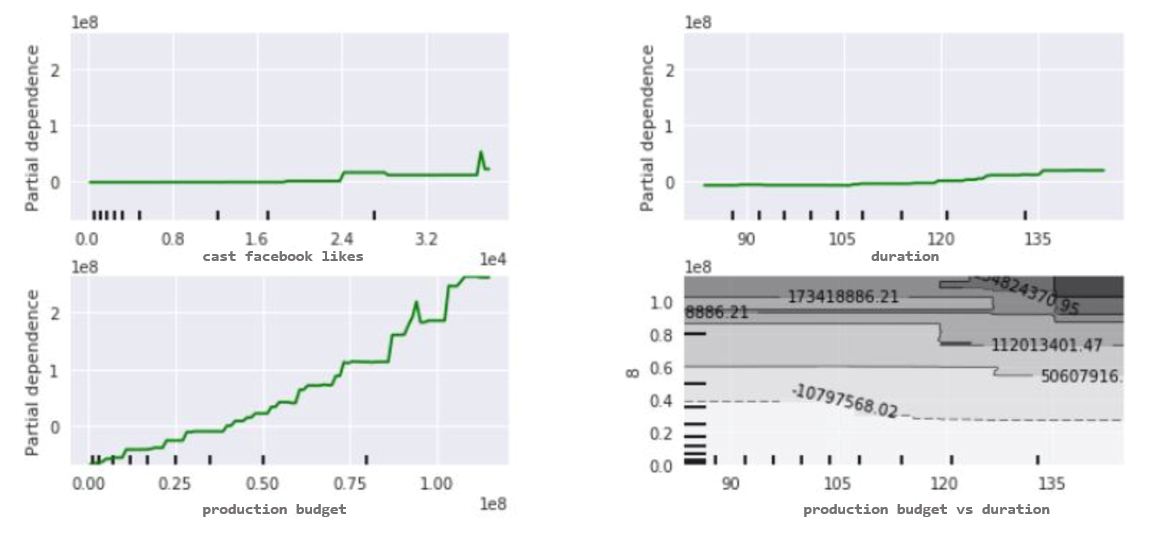
\includegraphics[width=3.2in]{figures/gradient_boost_dependency_}
\caption{Dependency Plot for Gradient Boosting Model} 
\label{fig:figgradientdep}
\end{figure}
\section{Classification}
CHECK THIS
Over 20 different classifiers have been used within the pipeline. As result of experimentation pipeline had been narrowed down to 3 classifiers: Logistic Regression, Neural Networks and Gradient Boosting.

Gradient boosting regressor has been found to be the best performing classifier for all classification cases. This section discusses the parameters optimization for growing the decisions trees and constructing the ensembles to generalize a well fitted model, taking into account bias/variance trade-off [1].

\begin{figure}[h]
\centering
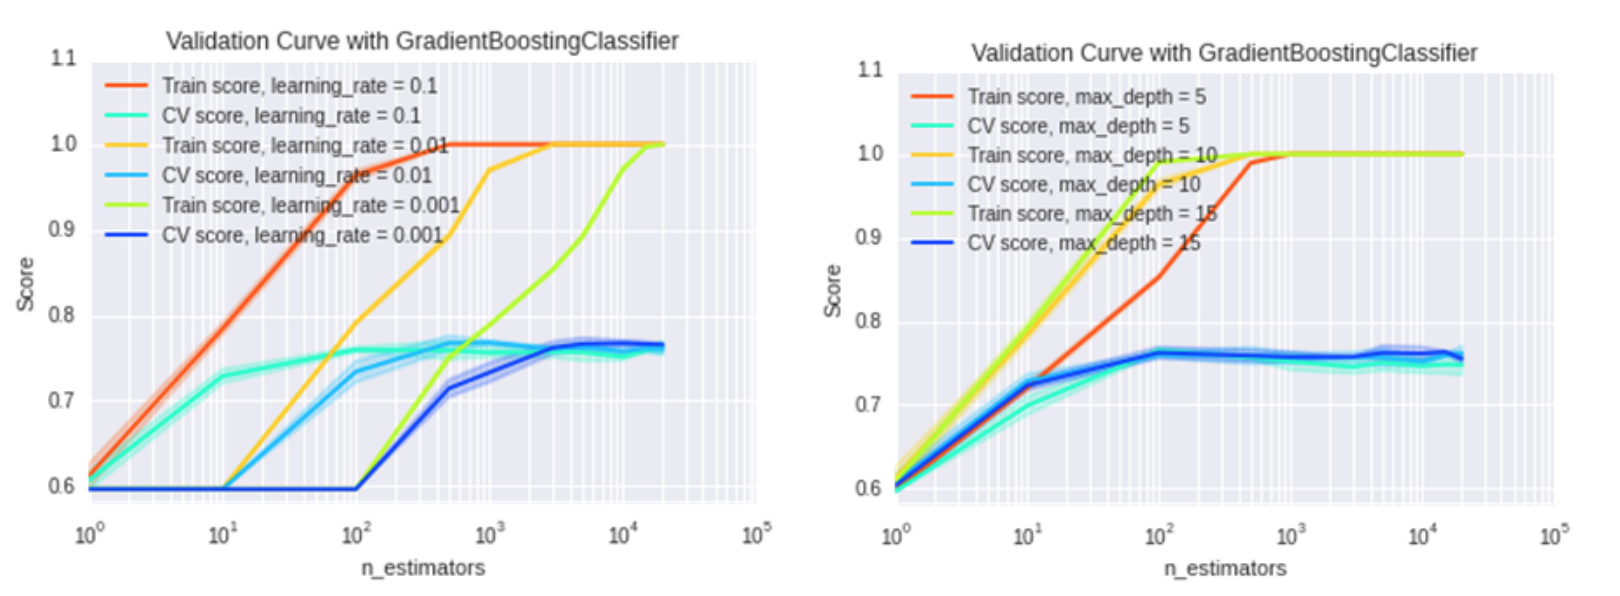
\includegraphics[width=3.2in]{figures/gb1}
\caption{GB1}
\label{fig:gb1}
\end{figure}
\begin{figure}[h]
\centering
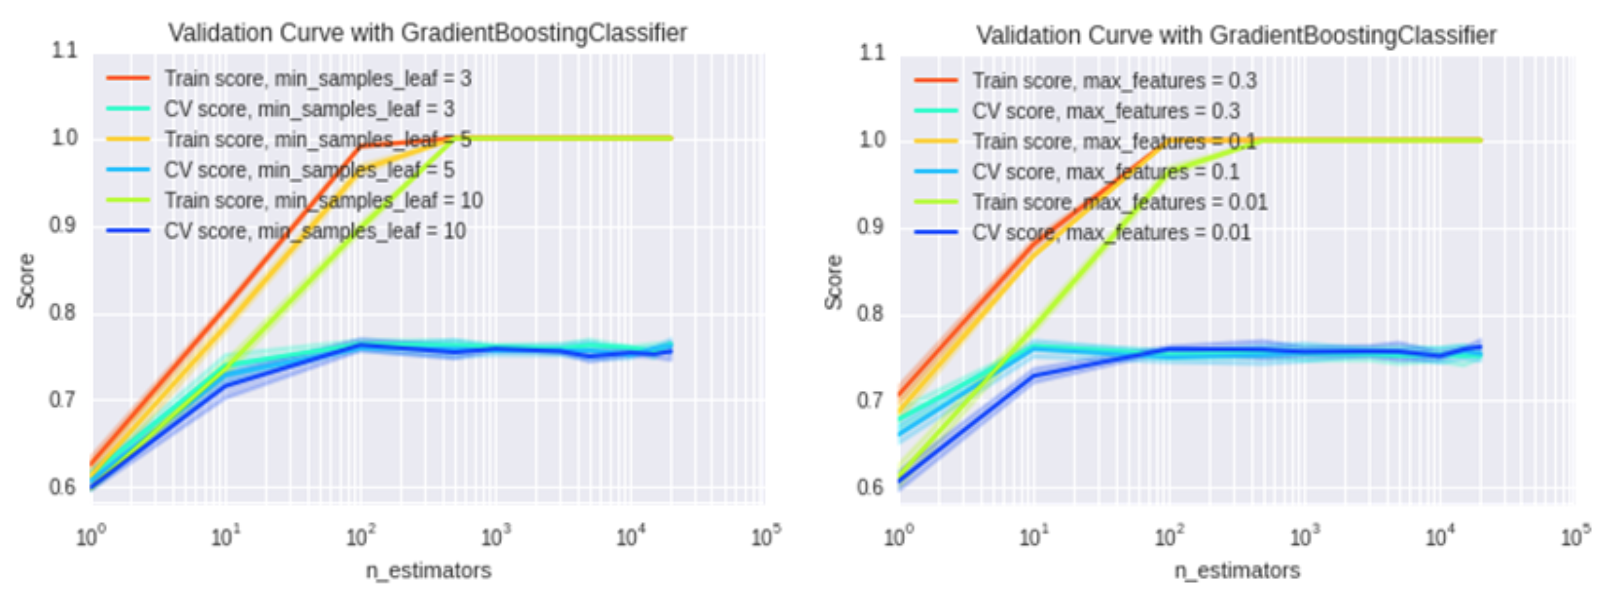
\includegraphics[width=3.2in]{figures/gb2}
\caption{GB2}
\label{fig:gb2}
\end{figure}
\begin{figure}[h]
\centering
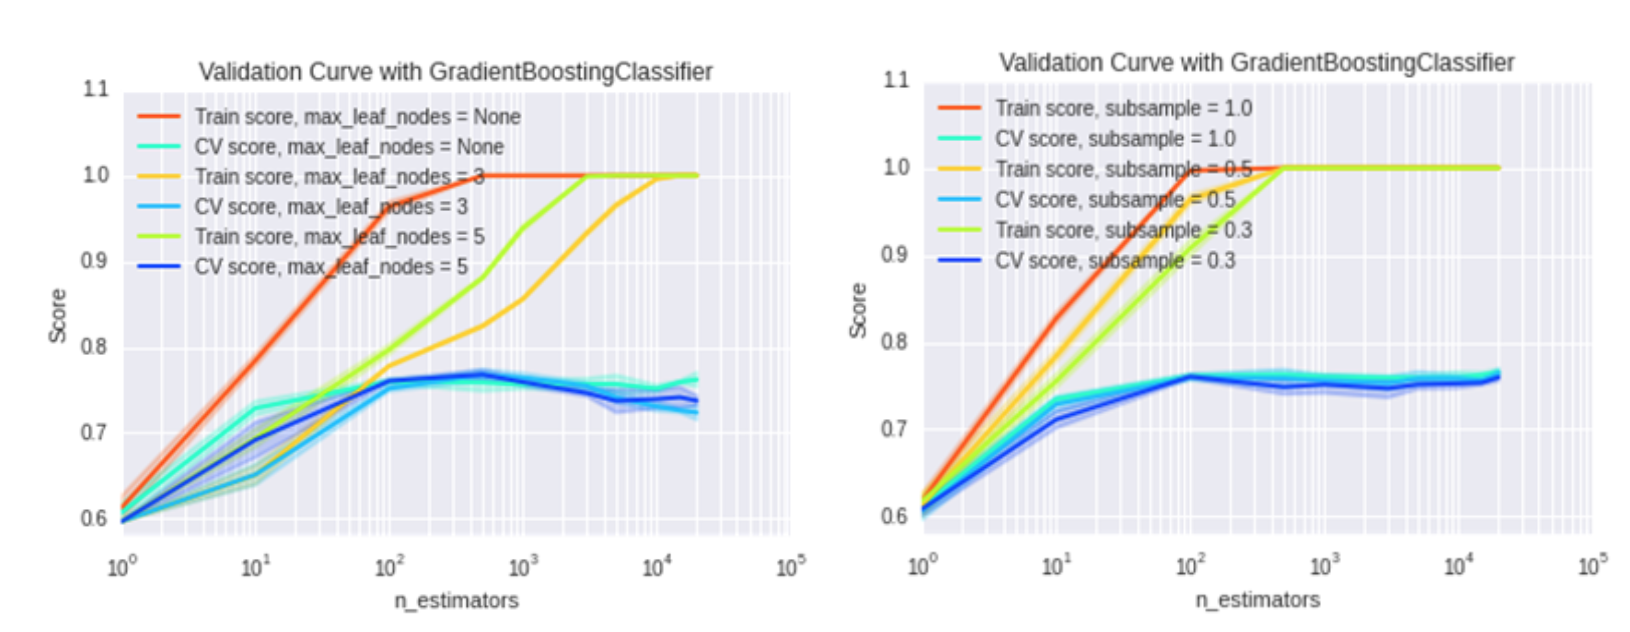
\includegraphics[width=3.2in]{figures/gb3}
\caption{GB3}
\label{fig:gb3}
\end{figure}

The learning rate/shrinkage represents the weight that is applied to the error minimization amount by each newly added decision tree [1]. As result a smaller learning rate requires more estimators to be added in order to more generalized model, as it can be seen in Figure 1. Learning rate of 0.01 achieves the highest performance with a small amount 500 ensembles and does not overcomplicate model as 0.001 rate. Max tree depth controls the maximal number of nodes within single tree, hence limiting number of decision a single tree can take. Max depth of 10 achieves an optimal performance with 100 ensembles. It can be seen that a bigger increase does not increase validation accuracy and only complicates the learning.  Min samples per leaf regulate the amount of samples necessary to fall within a node so that it becomes a leaf. Experimentation shows that having less than 3 samples per a leaf decreases the validation accuracy and lead to gain in variance.  Maximum features dictate the number of features to consider when classification tree looks for the best split in the samples provided in order to minimise the classification error [3]. The score of 0.1 of all features to be considered when split is produced produces a better generalising model. Max leaf nodes determine how many leafs can tree have when it is constructed, hence controls the amount of eventual decisions that are taken in the tree. No limit indicates unlimited amount of leafs and display the optimal performance.  Subsamples indicate the number of samples to be used to fit the individual trees in the ensemble. If amount of subsamples if less than 1.0 (all samples used) it results in a stochastic gradient boosting, which means that each next ensemble is trained with arbitrary different set of samples. Our results show that using all samples for minimizing the error leads to the best results.

\begin{figure}[h]
\centering
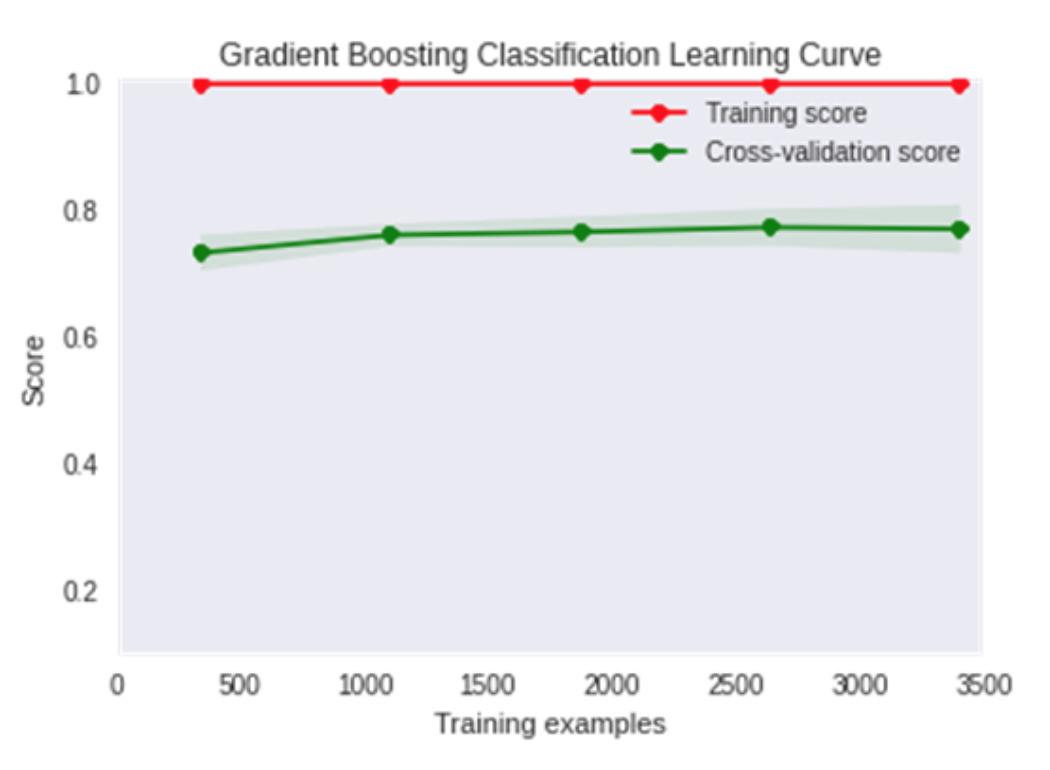
\includegraphics[width=3.2in]{figures/gb_learningcurve}
\caption{GB Learning curve}
\label{fig:learningcurve}
\end{figure}

Learning curve indicates the amount of data necessary to train a model up its maximal capability. It can be seen that Gradient Boosting Classifiers Requires over 3000
The analytical results coincide with findings of the parameters search over the pipeline ,which is \begin{verbatim}(max_leaf_nodes = None, learning_rate = 0.1,
max_depth =  10, min_samples_leaf = 5, 
max_features = 0.01, subsample = 1.0) \end{verbatim}­ This model has a good bias/variance balance, which produces a well generalising model.

\subsection{Final Model}
Two architectures were tested for the final model, which performs unification of classification and regression models, in order to improve regression accuracy. To optimize the model, a custom GridsearchCV function was written in order to support two models in a pipeline, unlike sklearn’s default of one. The first model trains a pipeline for the classification stage, which then concatenates its results with features for each data sample. Then a separate regression pipeline is trained from the concatenated samples, which then output final result.


The second model firstly is trained to classify all the samples and then for each set of classes produces an independent regression model. As a result, each gross class of samples uses a different optimized regression pipeline to find the final results.


\begin{figure}[h]
\centering
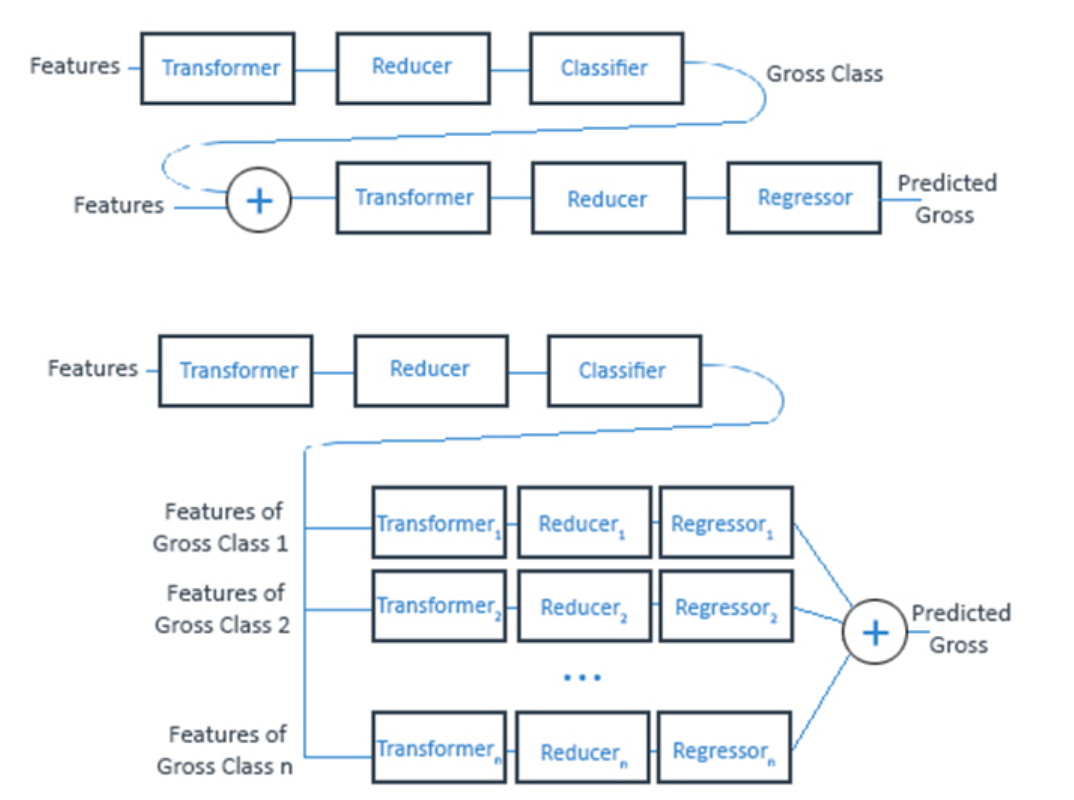
\includegraphics[width=3.2in]{figures/final_model}
\caption{Final model}
\label{fig:finalmodel}
\end{figure}

The second model was found to perform worse, due to much smaller training data available and as it was seen before, a gradient boost regression requires over 3000 samples to achieve validation saturation, but the average set size of classified samples available for training each regression step  ranges from 1920 down to 427.


\section{Results}
The followings results have been obtained from feeding the data through the first architecture of the final model. The table contains results for 9 different classification cases. It has to be noted that the sole regression results are indicated for comparison purposes and pure regression without class data fed in was not involved in generating the final result, whereas the classification results indicate the performance of the classification step of model, results of which are fed into the regression step.


\begin{table*}[!t]
\caption{LABEL. Class - score of the classification stage. Reg - reference score of the best standalone regression model. Combo - the regression results of the combined final model. Train - training accuracy, Valid - Cross validation accuracy, Test - Testing Accuracy. The classification results are measures as a fraction of classes predicted right. Regression results are measured as a R\^2 metric.}
\label{tab:top_ten_methods}
\centering
\begin{tabular}{|c|c|c|c|c|c|c|c|c|c|}
\hline
Classes & Class Train& Class Valid& Class Test& Reg Train& Reg Valid& Reg Test& Combo Train& Combo Valid& Combo Test \\
\hline
2 & 0.982 & 0.924 & 0.916 & 0.809 & 0.583 & 0.625 & 0.957 & 0.664 & 0.676 \\
3 & 0.872 & 0.761 & 0.771 & 0.809 & 0.583 & 0.625 & 0.906 & 0.669 & 0.691 \\ 
4 & 0.850 & 0.624 & 0.627 & 0.809 & 0.583 & 0.625 & 0.913 & 0.687 & 0.680 \\
5 & 0.868 & 0.536 & 0.549 & 0.809 & 0.583 & 0.625 & 0.723 & 0.690 & 0.670 \\
6 & 0.834 & 0.490 & 0.493 & 0.809 & 0.583 & 0.625 & 0.758 & 0.720 & 0.691 \\
7 & 0.839 & 0.461 & 0.479 & 0.809 & 0.583 & 0.625 & 0.772 & 0.746 & 0.679 \\
8 & 0.612 & 0.362 & 0.385 & 0.809 & 0.583 & 0.625 & 0.914 & 0.690 & 0.685 \\
9 & 0.642 & 0.356 & 0.377 & 0.809 & 0.583 & 0.625 & 0.844 & 0.700 & 0.681 \\
10 & 0.619 & 0.334 & 0.382 & 0.809 & 0.583 & 0.625 & 0.716 & 0.682 & 0.682 \\
\hline

\end{tabular}
\end{table*}


Class - score of the classification stage. Reg - reference score of the best standalone regression model. Combo - the regression results of the combined final model. Train - training accuracy, Valid - Cross validation accuracy, Test - Testing Accuracy. The classification results are measures as a fraction of classes predicted right. Regression results are measured as a R\^2 metric. 


\section{Discussion}
Our test results show that we can forecast a final gross of a movie with 69.1\%  when the final combinatory model is used. There are multiple class cases that equal this or get close to it, but only the case with 6 classification categories achieves a good general model. This case achieves 75.8\% training accuracy and 72\% cross validation score. Since these three scores are close in value, it indicates that model is neither under fitted or overfitted, and sits on an optimal point of the bias/variance tradeoff curve. It can observed that the combined model increases the regression validation and test performance by 13.8\%  and 6.6\% respectively. 

The gradient boosting has been found to be the best performing method for both classification and regression under same experimentation conditions (compared to Linear and Logistic regression, Support Vector Machines, Neural Networks). 

In the data transformation parts of the pipeline we have experimented with multiple logarithmic and polynomial, as well as standardisation and  normalization transforms. We have found that the most meaningful transform  is the logarithmical budget transform, which decreases the heteroscedasticity and improves the result, due to the budget explaining the most variance in the gross. Standardisation has been proven to improve results by near negligible  amount, as when data samples are split by the decision trees, feature scaling does not affect split area selection \cite{chen2014introduction}. Moreover, it was found that prior features selection in the model improves result only by  2-3\%, due to the fact gradient boosted trees perform the features selection implicitly during the ensemble process. 

Why it works better
As shown earlier, the gradient boosted trees can be easily trained to have near 100\% train accuracy by adding more tree ensembles. Using small amount of data with big amount of ensembles leads to overfitting. In our case using more than 500 ensembles leads to increase in variance and decreases cross-validation and  test scores. As a result, our model could be improved by simply using more training data. The gradient boosted model architecture could be empowered by using more regularized model formalization, also know as 'xgboost'. This allows for a better control over overfitting, by penalizing complex models, hence makes the model to learn a better objective function faster \cite{chen2015}.  

It is important to note that the performance was significantly improved during the feature engineering phase. Initial model runs had scored more than 10\% lower than the final results. Some patterns were noticed, for example the length of movies is strongly correlated with the box office performance. Popular movies, like Lord of the Rings Trilogy, Avatar, Titanic, all have high grosses and long running times. The dataset had outliers that had running times more than 300 minutes. The longest movie run for 511 minutes,  and eliminating occurrences like this helped models. Data cleaning had a similar effect as well, especially the removal of empty values and fixing of the currency issue.

Other studies have also faced the problem of box-office prediction with features available only before the launching of a movie. The accuracy obtained here is better than that obtained in \cite{zhang2009forecasting}, where Zhang et. al. obtained 68.1\% accuracy predicting box office income in a 6-class classification problem using multi-layer BP neural network (MLBP) through 6-fold cross validation. The first paper facing the problem of predicting box-office success before theatrical release \cite{sharda2006predicting}, accomplished a modest absolute prediction accuracy of only 36.9\% on a 9-class classification problem using 10-fold cross validation. 



\section{Conclusion}